
\section{Non-homogeneous Poisson Process}

The account selected for the extraction of the tweets is \textit{@realmadrid} since it has a constant number of retweets (RT), not extremely high, allowing us to measure the counting process in a reasonable time space. Although library \textit{rtweet} obtains information about the retweets and their time stamps it is worth mentioning that the results detailed here do not reflect the actual behaviour of the account since retweet count is limited to 100.

\subsection{Use descriptive statistics and graphics to explore the retweets data set in terms of the number of retweets by time and the time between retweets. Does it fit the hypothesis of a Poisson process?}

We know that a Poisson process is a counting process related with the Poisson and Exponential distributions. Being a counting process a stochastic process $\mathbf{N} = \{ N_t, t \geq 0 \}$ satisfying:
\begin{itemize}
	\item $N_t=0$
	\item $N_t$ is integer valued
	\item For $s<t, N_s \leq N_t$
	\item For $s<t, N_t - N_s$ represents the number of events that occur in the time intervals (s, t]
\end{itemize}

When plotting the tweet with maximum retweets (limited) we can see the behaviour of the retweet counting process.
\begin{figure}[H]
	\centering
	% Created by tikzDevice version 0.12.3 on 2019-12-18 11:55:35
% !TEX encoding = UTF-8 Unicode
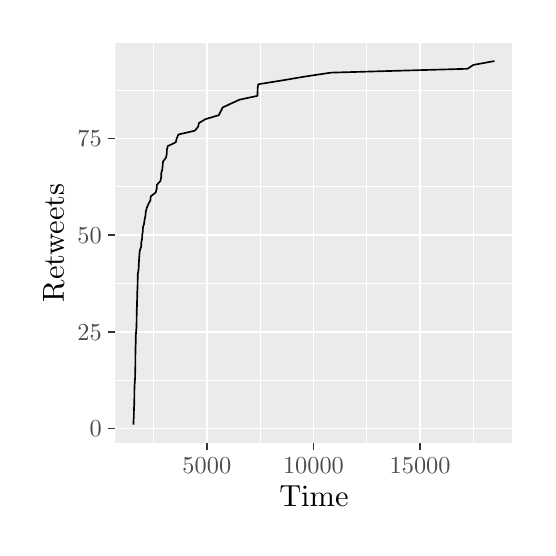
\begin{tikzpicture}[x=1pt,y=1pt]
\definecolor{fillColor}{RGB}{255,255,255}
\path[use as bounding box,fill=fillColor,fill opacity=0.00] (0,0) rectangle (180.67,180.67);
\begin{scope}
\path[clip] (  0.00,  0.00) rectangle (180.67,180.67);
\definecolor{drawColor}{RGB}{255,255,255}
\definecolor{fillColor}{RGB}{255,255,255}

\path[draw=drawColor,line width= 0.6pt,line join=round,line cap=round,fill=fillColor] (  0.00,  0.00) rectangle (180.68,180.68);
\end{scope}
\begin{scope}
\path[clip] ( 31.71, 30.69) rectangle (175.17,175.17);
\definecolor{fillColor}{gray}{0.92}

\path[fill=fillColor] ( 31.71, 30.69) rectangle (175.17,175.17);
\definecolor{drawColor}{RGB}{255,255,255}

\path[draw=drawColor,line width= 0.3pt,line join=round] ( 31.71, 53.32) --
	(175.17, 53.32);

\path[draw=drawColor,line width= 0.3pt,line join=round] ( 31.71, 88.26) --
	(175.17, 88.26);

\path[draw=drawColor,line width= 0.3pt,line join=round] ( 31.71,123.19) --
	(175.17,123.19);

\path[draw=drawColor,line width= 0.3pt,line join=round] ( 31.71,158.13) --
	(175.17,158.13);

\path[draw=drawColor,line width= 0.3pt,line join=round] ( 45.47, 30.69) --
	( 45.47,175.17);

\path[draw=drawColor,line width= 0.3pt,line join=round] ( 84.00, 30.69) --
	( 84.00,175.17);

\path[draw=drawColor,line width= 0.3pt,line join=round] (122.54, 30.69) --
	(122.54,175.17);

\path[draw=drawColor,line width= 0.3pt,line join=round] (161.07, 30.69) --
	(161.07,175.17);

\path[draw=drawColor,line width= 0.6pt,line join=round] ( 31.71, 35.86) --
	(175.17, 35.86);

\path[draw=drawColor,line width= 0.6pt,line join=round] ( 31.71, 70.79) --
	(175.17, 70.79);

\path[draw=drawColor,line width= 0.6pt,line join=round] ( 31.71,105.73) --
	(175.17,105.73);

\path[draw=drawColor,line width= 0.6pt,line join=round] ( 31.71,140.66) --
	(175.17,140.66);

\path[draw=drawColor,line width= 0.6pt,line join=round] ( 64.74, 30.69) --
	( 64.74,175.17);

\path[draw=drawColor,line width= 0.6pt,line join=round] (103.27, 30.69) --
	(103.27,175.17);

\path[draw=drawColor,line width= 0.6pt,line join=round] (141.80, 30.69) --
	(141.80,175.17);
\definecolor{drawColor}{RGB}{0,0,0}

\path[draw=drawColor,line width= 0.6pt,line join=round] ( 38.23, 37.25) --
	( 38.25, 38.65) --
	( 38.36, 40.05) --
	( 38.38, 41.45) --
	( 38.40, 42.84) --
	( 38.49, 44.24) --
	( 38.51, 45.64) --
	( 38.55, 47.04) --
	( 38.56, 48.43) --
	( 38.57, 49.83) --
	( 38.62, 51.23) --
	( 38.70, 52.62) --
	( 38.81, 54.02) --
	( 38.83, 55.42) --
	( 38.87, 56.82) --
	( 38.90, 58.21) --
	( 38.92, 59.61) --
	( 38.92, 61.01) --
	( 38.93, 62.41) --
	( 38.95, 63.80) --
	( 38.97, 65.20) --
	( 39.04, 66.60) --
	( 39.04, 68.00) --
	( 39.06, 69.39) --
	( 39.19, 70.79) --
	( 39.29, 72.19) --
	( 39.34, 73.59) --
	( 39.37, 74.98) --
	( 39.38, 76.38) --
	( 39.43, 77.78) --
	( 39.44, 79.17) --
	( 39.52, 80.57) --
	( 39.53, 81.97) --
	( 39.57, 83.37) --
	( 39.58, 84.76) --
	( 39.66, 86.16) --
	( 39.72, 87.56) --
	( 39.74, 88.96) --
	( 39.76, 90.35) --
	( 39.80, 91.75) --
	( 40.06, 93.15) --
	( 40.13, 94.55) --
	( 40.18, 95.94) --
	( 40.29, 97.34) --
	( 40.38, 98.74) --
	( 40.51,100.14) --
	( 41.01,101.53) --
	( 41.02,102.93) --
	( 41.33,104.33) --
	( 41.38,105.73) --
	( 41.63,107.12) --
	( 41.65,108.52) --
	( 42.08,109.92) --
	( 42.24,111.31) --
	( 42.56,112.71) --
	( 42.66,114.11) --
	( 43.04,115.51) --
	( 43.60,116.90) --
	( 44.36,118.30) --
	( 44.46,119.70) --
	( 46.26,121.10) --
	( 46.62,122.49) --
	( 46.71,123.89) --
	( 47.98,125.29) --
	( 48.24,126.69) --
	( 48.27,128.08) --
	( 48.65,129.48) --
	( 48.78,130.88) --
	( 48.90,132.28) --
	( 49.97,133.67) --
	( 50.25,135.07) --
	( 50.30,136.47) --
	( 50.62,137.86) --
	( 53.50,139.26) --
	( 53.86,140.66) --
	( 54.48,142.06) --
	( 60.42,143.45) --
	( 61.57,144.85) --
	( 61.92,146.25) --
	( 64.33,147.65) --
	( 69.07,149.04) --
	( 69.76,150.44) --
	( 70.46,151.84) --
	( 73.47,153.24) --
	( 76.50,154.63) --
	( 83.02,156.03) --
	( 83.07,157.43) --
	( 83.10,158.83) --
	( 83.32,160.22) --
	( 92.03,161.62) --
	(100.30,163.02) --
	(109.60,164.42) --
	(158.92,165.81) --
	(161.06,167.21) --
	(168.65,168.61);
\end{scope}
\begin{scope}
\path[clip] (  0.00,  0.00) rectangle (180.67,180.67);
\definecolor{drawColor}{gray}{0.30}

\node[text=drawColor,anchor=base east,inner sep=0pt, outer sep=0pt, scale=  0.88] at ( 26.76, 32.83) {0};

\node[text=drawColor,anchor=base east,inner sep=0pt, outer sep=0pt, scale=  0.88] at ( 26.76, 67.76) {25};

\node[text=drawColor,anchor=base east,inner sep=0pt, outer sep=0pt, scale=  0.88] at ( 26.76,102.69) {50};

\node[text=drawColor,anchor=base east,inner sep=0pt, outer sep=0pt, scale=  0.88] at ( 26.76,137.63) {75};
\end{scope}
\begin{scope}
\path[clip] (  0.00,  0.00) rectangle (180.67,180.67);
\definecolor{drawColor}{gray}{0.20}

\path[draw=drawColor,line width= 0.6pt,line join=round] ( 28.96, 35.86) --
	( 31.71, 35.86);

\path[draw=drawColor,line width= 0.6pt,line join=round] ( 28.96, 70.79) --
	( 31.71, 70.79);

\path[draw=drawColor,line width= 0.6pt,line join=round] ( 28.96,105.73) --
	( 31.71,105.73);

\path[draw=drawColor,line width= 0.6pt,line join=round] ( 28.96,140.66) --
	( 31.71,140.66);
\end{scope}
\begin{scope}
\path[clip] (  0.00,  0.00) rectangle (180.67,180.67);
\definecolor{drawColor}{gray}{0.20}

\path[draw=drawColor,line width= 0.6pt,line join=round] ( 64.74, 27.94) --
	( 64.74, 30.69);

\path[draw=drawColor,line width= 0.6pt,line join=round] (103.27, 27.94) --
	(103.27, 30.69);

\path[draw=drawColor,line width= 0.6pt,line join=round] (141.80, 27.94) --
	(141.80, 30.69);
\end{scope}
\begin{scope}
\path[clip] (  0.00,  0.00) rectangle (180.67,180.67);
\definecolor{drawColor}{gray}{0.30}

\node[text=drawColor,anchor=base,inner sep=0pt, outer sep=0pt, scale=  0.88] at ( 64.74, 19.68) {5000};

\node[text=drawColor,anchor=base,inner sep=0pt, outer sep=0pt, scale=  0.88] at (103.27, 19.68) {10000};

\node[text=drawColor,anchor=base,inner sep=0pt, outer sep=0pt, scale=  0.88] at (141.80, 19.68) {15000};
\end{scope}
\begin{scope}
\path[clip] (  0.00,  0.00) rectangle (180.67,180.67);
\definecolor{drawColor}{RGB}{0,0,0}

\node[text=drawColor,anchor=base,inner sep=0pt, outer sep=0pt, scale=  1.10] at (103.44,  7.64) {Time};
\end{scope}
\begin{scope}
\path[clip] (  0.00,  0.00) rectangle (180.67,180.67);
\definecolor{drawColor}{RGB}{0,0,0}

\node[text=drawColor,rotate= 90.00,anchor=base,inner sep=0pt, outer sep=0pt, scale=  1.10] at ( 13.08,102.93) {Retweets};
\end{scope}
\end{tikzpicture}

	\vspace*{-0.9em}
	\caption{Tweet with maximum RT process}
\end{figure}